\documentclass[
	10pt,
	parskip=half-,	
	paper=a4,
	english
	]{scrartcl}	
\usepackage{graphicx} % Required for inserting images
\usepackage{datetime}

\usepackage[english]{babel} 
\textheight = 220mm		
\footskip = 2cm		
\title{Title of the project}
\author{Author}
\date{\newdateformat{monthyeardate}{%
  \monthname[\THEMONTH], \THEYEAR}}

\usepackage{algorithm}
\usepackage{algpseudocode}
\usepackage{subcaption}
\usepackage{caption}
\usepackage{amsmath}
\usepackage{amssymb}
\usepackage{hyperref}
\hypersetup{
    colorlinks=true,
    linkcolor=black,
    filecolor=magenta,      
    urlcolor=blue,
    pdftitle={projectname},
}
\usepackage{fancyhdr}
\usepackage{booktabs}
\pagestyle{fancy}
\lhead{AC via maximum incremental path integral}
\rhead{Bernat Comas}
\date{}

\begin{document}

\begin{titlepage}
    \centering
    \vspace*{\fill}

    {\Huge\bfseries Agglomerative clustering via maximum incremental path integral: an implementation}
    \vspace{1cm}
    
    {\bfseries Unsupervised and Reinforcement Learning\\} % Second line of the title
    \vspace{0.5cm}
    {\bfseries \today}
    \vspace{1.5cm}

    {\Large Bernat Comas i Machuca}
    \vspace{0.5cm}

    {\Large \date{\newdateformat{monthyeardate}{%
  \monthname[\THEMONTH], \THEYEAR}}}

    \vspace*{\fill} % Vertically center the content

\end{titlepage}

\newpage			
\tableofcontents
\newpage
\section {Introduction to the problem}

The paper Agglomerative clustering via maximum incremental path integral (2013) \cite{citation1} presents a new agglomerative clustering algorithm that computes cluster similarity based on path graphs that capture the data structure. To make this computation each cluster is treated as a dynamic system and the algorithm measures stability using the Path Integral, a concept extracted from statistical mechanics and quantum mechanics. In doing so, it introduces a novel hierarchical clustering approach by rethinking how to measure the similarity between clusters during the agglomerative process.

To define the structural descriptors that allow to compute this concept of similarity, a neighborhood graph is created. This allows it to avoid relying as much in pairwise distances (only used for graph initialization), and instead define the affinity between clusters by how much their stability changes when merged, which is measured through the path integral.

This has several advantages:

\begin{itemize}
    \item Works well for data lying on low-dimensional manifolds.
    \item It does not rely on approximation or eigen-decomposition, making it more robust to noise.
    \item It does not make assumptions on data distribution, offering better generalization.
    \item Performs well on multi-scale data
    \item It is efficiently computed by the presented algorithm in linear time complexity
\end{itemize}

Over the course of this project, we are going to implement the Path Integral Clustering algorithm in an efficient way, and then we are going to compare it to other well-known clustering algorithms. In this section we are going to describe the algorithm, section 2 contains a description of the implementation , in section 3 the algorithm experiments and comparison is performed, and finally the last section is devoted to describing the conclusions of the project.

\subsection{Novelty of the Path Integral Clustering}

This paper presents a new approach to agglomerative clustering, which is a popular method for hierarchical clustering. The novelty lies in the way it defines inter-cluster similarity and the algorithmic approach to compute it. It can be summed up in:

\begin{enumerate}
    \item Defining a new linkage criterion based on a path integral formulation: Instead of typical linkage methods like single-link, complete-link, or average-link, which rely on direct distance metrics between points or clusters, this method computes the maximum incremental path integral (MIPI) between clusters.
    
    \item The "path integral" represents the cumulative similarity (or affinity) along the path connecting two clusters through a series of intermediate points. In this way, the method captures both local and global structure information in the dataset, which is an evolution from pairwise distances.
    
    \item The MIPI criterion considers not just the shortest path between clusters, but the maximum incremental contribution a new link would make to the total path integral when merging clusters. This ensures clusters are merged in a way that preserves high-density connections and prevents weakly connected or noisy points from dominating cluster formation.
\end{enumerate}

This is particularly useful as it balances local density and global connectivity, making it more robust in dealing with datasets where traditional linkage-based hierarchical clustering struggles, such as datasets with complex shapes or varying densities, noisy data, non-convex clusters, or when the distance metric alone isn't enough to capture cluster structure.

\subsection{Cluster initialization}

Because we are working with an Agglomerative Clustering algorithm, we have to define how will the initial clusters be formed. We could initialize the samples each in its own cluster and start the iteration, but instead the paper proposes to use nearest neighbor merging. 

The algorithm of nearest neighbor merging consists of having each sample in its own cluster together with its nearest neighbor and then, the clusters that share samples are merged. This results in a number of initial clusters that is at least half the number of samples.

\subsection{Building the structural graph}

We define the structural graph G as the directed graph where each initial sample X is a node and E the set of edges connecting them. Two samples are connected by an edge if they are in its K closest neighbors (for a predefined graph).

Then, we compute the weighted adjacency matrix W, which contains the pairwise similarities between each pair of samples. Note that we are only computing similarities between each point and its K closest neighbors, the rest of similarities will be 0. Therefore, each element \(w_ij)\) of the matrix W is defined as shown in Equation \ref{eq1}.

\begin{equation}
    w_{ij} =
    \begin{cases} 
    \exp \left( \frac{-\text{dist}(i,j)^2}{\sigma^2} \right), & \text{if } \mathbf{x}_j \in \mathcal{N}_i^K, \\
    0, & \text{otherwise}.
    \end{cases}
    \label{eq1}
\end{equation}

Where \textit{K} is a free parameter to be set and \(\sigma^2\) is estimated by Equation \ref{eq4}.

\begin{equation}
    \sigma^2 = [\sum_{j=1}^{n}\sum_{x_j\in \mathcal{N}_i^3}dist(i,j)^2] / [3n(-ln(a))]
    \label{eq4}    
\end{equation}

Where \textit{a} is a parameter to be set.

We define the transition probability matrix \textit{P} as the one-step transition probability from vertex i to vertex j, and we compute it using Equation \ref{eq5}.

\begin{equation}
    \begin{split}
    P = D^{-1}W; 
    \\
    d_{ii} = \sum_{j=1}^n w_{ij}
    \text{ such that }
    \sum_{j=1}^n p_{ij}=1
    \end{split}
    \label{eq5}
\end{equation}

\subsection{Affinity measure: Path integral}

The path integral of a cluster is computed by summing the paths in the cluster on the directed graph \textit{G}, weighted by transition probabilities in \textit{P}.

The path integral used is a discretization of the one seen in quantum mechanics, and is defined as a sum of the weighted contributions of all the paths in the cluster C, divided by the number of samples belonging to the cluster. This is called the path integral descriptor of a cluster \(C_a\), which we call \(S_{C_a}\), and is defined in Equation \ref{eq2}.
\ref{eq2}.

\begin{equation}
    S_c = \frac{1}{|C|^2}\sum_{\gamma\in\Gamma_c}{\Theta(\gamma)}
\label{eq2}
\end{equation}

Where, \(\Gamma_c\) is the set of all paths in C and \(\Theta(\gamma)\) the weight of a path.

We also define the conditional path integral descriptor \(S_{C_a|C_a\cup C_b}\) between two clusters \(S_{C_a}\) and \(S_{C_b}\) as the path descriptor of the clustering resulting from the merge but only taking into account the paths that have starting and ending vertices in \(C_a\). We compute the conditional path integral descriptor using Equation \ref{eq6}.

\begin{equation}
    S_{C_a|C_a\cup C_b} = \frac{1}{|C_a|^2} \boldsymbol{1}_{C_a}^{T}(\boldsymbol{I}-z\boldsymbol{P}_{C_a\cup C_b})^{-1}\boldsymbol{1}_{C_a}
    \label{eq6}
\end{equation}

Now, we can compute the affinity \(A_{C_a,C_b}\) of the merging of two clusters \(C_a\) and \(C_b\) by the increment in the path integral descriptor shown in the previous equations \ref{eq2} and \ref{eq6}, as can be seen in Equation \ref{eq3}. In addition to the path integral of each cluster separately \(S_{C_a}\) and \(S_{C_b}\), the computation of the affinity uses the conditional path integral descriptor \(S_{C_a|C_a\cup C_b}\), which computes the resulting path descriptor of the merge but only the ones that have starting and ending vertices in \(C_a\).

\begin{equation}
    A_{C_a,C_b} = (S_{C_a|C_a\cup C_b}-S_{C_a}) + (S_{C_b|C_a\cup C_b}-S_{C_b})
    \label{eq3}
\end{equation}

\subsection{Agglomerative algorithm}

The input to our problem is a set of sample vectors together with the target number of clusters (that has to be predefined).

The algorithm starts by building the graph, weighted adjacency matrix \(W\), and using it to obtain the transition probability matrix \(P\). Then, cluster initialization is run to obtain the initial clusters.

The iterative part consists of merging the two most affine clusters we have until the number of clusters is the target one. To do so, we use the precomputed affinities between all pairs of clusters. % The pseudocode of the algorithm can be seen in Algorithm \ref{algorithmpseudo}.

% \begin{algorithm}
% \caption{Path Integral Clustering Algorithm}
% \begin{algorithmic}[1]
%     \State \textbf{INPUT} The set of $n$ points to cluster $\mathcal{X} = \{\mathbf{x}_1, \mathbf{x}_2, \dots, \mathbf{x}_n\}$, and the target number of clusters $n_T$.
%     \State Build the graph $G$ with $k$-nearest-neighbors and compute its weighted adjacency matrix $\mathbf{W}$.
%     \State Get the transition probability matrix $\mathbf{P}$
%     \State Run nearest neighbour merging to form $n_c$ initial clusters $\mathcal{C}_c = \{\mathcal{C}_1, \ldots, \mathcal{C}_{n_c}\}$.
%     \While{$n_c > n_T$}
%         \State Search two clusters $\mathcal{C}_a$ and $\mathcal{C}_b$, such that 
%         \[
%         \{\mathcal{C}_a, \mathcal{C}_b\} = \arg\max_{\mathcal{C}_a, \mathcal{C}_b \in \mathcal{C}_c} \mathcal{A}_{\mathcal{C}_a, \mathcal{C}_b}
%         \]
%         where $\mathcal{A}_{\mathcal{C}_a, \mathcal{C}_b}$ is the affinity measure between $\mathcal{C}_a$ and $\mathcal{C}_b$.
%         \State $\mathcal{C}_c \leftarrow \{\mathcal{C}_c \setminus \{\mathcal{C}_a, \mathcal{C}_b\} \} \cup \{\mathcal{C}_a \cup \mathcal{C}_b\}$
%         \State $n_c \leftarrow n_c - 1$
%     \EndWhile
%     \State \textbf{OUTPUT} $\mathcal{C}_c$
% \end{algorithmic}
% \label{algorithmpseudo}
% \end{algorithm}

\newpage
\section {Description of the implementation}

In this section we are going to describe the particularities of the implementation of the Path Integral Clustering Algorithm. The first section goes over the implementation techniques recommended by the paper, and the second one contains the extra decisions made during the implementation. 

During the implementation, efficiency was our priority. The full implementation of the algorithm is contained in the files \textit{"pic.py"}, \textit{"nearest\_neighbour\_init.py"} and \textit{"path\_integral.py"}. The rest of files are helpers that have contributed to the results obtained but are not part of the implementation itself.

\subsection{Efficient computation of the path integral}

The main ideas laid out by the paper about the implementation are on the computation of the path integral between two clusters. They use Theorem 1 to avoid computing a matrix inverse but instead solve a linear system. 

\textbf{Theorem 1}. $s_{ij}$ always converges, and $s_{ij}= \left[(I - zP_{\mathcal{C}})^{-1}\right]_{ij}$, i.e., the $(i,j)$-element of $(I-zP_{\mathcal{C}})^{-1}$, where $P_{\mathcal{C}}$ is the submatrix of $P$ by selecting the samples in $\mathcal{C}$. If we define $S_{\mathcal{C}} = [s_{ij}]_{i,j \in \mathcal{C}}$, we have $S_{\mathcal{C}} = (I - zP_{\mathcal{C}})^{-1}$. Then, we can compute the path integral as the structural descriptor of cluster $\mathcal{C}$ as follows:

\begin{equation}
    S_{\mathcal{C}} = \frac{1}{|\mathcal{C}|^2} \mathbf{1}^{T} S_{\mathcal{C}} \mathbf{1}
    = \frac{1}{|\mathcal{C}|^2} \mathbf{1}^{T} (I - zP_{\mathcal{C}})^{-1} \mathbf{1}
    \label{eq8}
\end{equation}

where $\mathbf{1}$ is all-one column vector.

\textbf{Proposition 1} $(I - zP_{\mathcal{C}})$ is a strictly diagonally dominant matrix with the $\infty$-norm condition number no more than $(1+z)/(1-z)$.

Both Theorem 1 and Proposition 1 are proven in the original paper \cite{citation1}, so we will not go into more detail here. Taking them into account, we see that the computation of $S_{\mathcal{C}}$ only involves solving a linear system

\begin{equation}
    \begin{split}
    (I - zP_{\mathcal{C}}) \mathbf{y} = \mathbf{1},
    \label{eq7}
    \\
    S_{\mathcal{C}} = \frac{1}{|\mathcal{C}|^2} \mathbf{1}^{T} \mathbf{y}.
    \end{split}
\end{equation}

For a large cluster, $(I - zP_{\mathcal{C}})$ is sparse, which means it follows Proposition 1 and can be solved using iterative methods. This will help us compute both the incremental path integral and the path integral descriptor.

\begin{equation}
    S_{c_a|c_a \cup c_b} = \frac{1}{|c_a|^2} \mathbf{1}_{c_a}^{T} (I - zP_{c_a \cup c_b})^{-1} \mathbf{1}_{c_a}
\end{equation}

To compute the path integral descriptor as shown in Equation \ref{eq8}, we first compute \((I - zP_{c_a \cup c_b})\), which is straightforward. Then, following equation \ref{eq7}, we solve the linear system (we can use spsolve). Finally, multiplying by the transposed matrix of 1s is the same as summing all the elements in the matrix resulting from the linear equation's solving, and finally we can compute the multiplication with the fraction. Computing the incremental path descriptor takes advantage of the same trick. 

\subsection{Implementation decisions}

Because we want our algorithm to run in linear time, we need to precompute everything we can, and that includes not only the graph and its transition matrices, but also the affinity between each pair of clusters. This is because we are going to be merging clusters in a greedy way, and we want to avoid having to compute the affinities at each iteration. We are going to compute the affinities between all pairs of clusters at the beginning, and then we will only need to update the ones that are affected by the merge. This is because when we merge two clusters, we only need to compute the affinities between the new cluster and all the previous ones, and not between all pairs of clusters.

In addition to this, we are using a heap to store all the cluster pairs and their affinities for fast extraction in runtime. This brought us to use a set to store the clusters that are active in a moment, to avoid having to traverse the heap to remove all pairs of clusters that contains one of the merged ones at each iteration. This means that at every iteration we are flagging the merged clusters as inactive, computing the affinities between the new cluster and all the previous ones, and adding them to the heap.

Due to the nature of our algorithm, we only implement the fit-predict method. This is because the algorithm does not learn from data but instead applies the same process to the samples to cluster them independently from the data it has seen.

Another decision we made to improve efficiency that was not stated in the paper is, because the algorithm always computes K-nearest-neighbours and also 3-nearest neighbours, we decided to use the same graph for both. This means that we are going to compute the K-nearest-neighbours graph and then we are going to use it to compute the 3-nearest-neighbours graph. This is because the 3-nearest-neighbours graph is a subset of the K-nearest-neighbours graph, and this can save us a lot of time. In addition to this, in the pairwise similarity matrix computation we also use the distances computed by the KNN algorithm to avoid having to compute them again.

All the operations that involve the clustering algorithm use numpy, using matrices as numpy arrays, and taking advantage of the different tools we have to work with sparse matrices. Because of the way the similarities are computed, being set to zero if they are not in the K nearest neighbors of every sample, and because of their enormous sizes, we use different tools from scipy.sparse, including spsolve to solve the linear systems that compute the Path Integral (see previous section), converting matrices to csc form and making computations between matrices using the sparse tools.

\section {Experiments}

In this section we will conduct experiments comparing different clustering algorithms on several datasets. The algorithms under evaluation include Affinity Propagation, Complete Link, Average Link, Simple Link, Zeta clustering (Zell), Difussion clustering, and of course, our implementation of PIC. Each algorithm will be tested on four datasets: MNIST, USPS, Breast Cancer (Wisconsin), and three differently-structured synthetic random datasets with 1000 samples each. We are going to divide the experiments section into several subsections. In the first subsection, we are going to talk about the metrics we are using to compare the models. In the second one, we are going to analyse the performance of the algorithms over the synthetic datasets. Next, we are going to run the algorithms on the complete datasets to observe what are the differences in their performances, using a diverse set of metrics. Finally, we are going to analyse how does the introduction of gaussian noise and structural noise affect the performance of the different algorithms, similar to what is done in the original paper.

The choice of the algorithms we are using is due to the fact that we only have found implementations for the Affinity Propagation, Complete, Average and Simple Links. Although in the project we only had to implement PIC, we decided to also implement some of the algorithms that get the most similar results in the paper, and the selected algorithms to implement are the diffusion Kernel (D-kernel) and Zeta function clustering (Zell), because they are shown to be better than PIC in some domains in the original paper. To do the PIC experiments, we are using exactly the same parameters recommended by the original paper, which are: \(K=20\), \(a=0.95\) and \(z=0.01\). The rest of the algorithms are using their default parameters, as we are not trying to tune them but rather compare them.

The datasets chosen are also extracted from the paper: MNIST and USPS. We opted not to use the FRGC ver2.0, PubFig, and Caltech datasets for this study due to their large size, which would require significant computational resources and time for processing, apart from the approach the paper takes on loading them, which uses spatial pyramid features. Instead, we have decided to incorporate the Breast-cancer wisconsin dataset because it is a well-known benchmark in the medical domain, containing a high-dimensional, real-world classification and being widely used. In addition, being a binary classification dataset, it stands out from the rest and means that the algorithms will have to iterate until only two clusters are remaining, apart from being something not tested in the original paper.

It is worth noting that in our work, we used the original USPS dataset containing 9,298 samples, rather than the 11,000-sample version referenced in the paper. We chose to work with the authentic USPS dataset, as the source and details of the augmented version with additional samples used by the paper were unclear.

We don't have access to the synthetic datasets that are used in the paper, and for this reason we have decided to create our own. It will be through the synthetic datasets that we will study how does structural and gaussian noise affect our implementation of the clustering algorithm. To have datasets as diverse as possible, we are going to use three different creation methods, the first one using moons, second one using concentric circles and last one using blobs. Our synthetic datasets will have 1000 samples, 2 features for ease of representation (same as the ones in the paper) and 10 target clusters.

\begin{table}[h]
\centering
\caption{Statistics of used datasets. Synthetic represents the three synthetic datasets: blobs, moons and circles.}
\begin{tabular}{lccccc}
\toprule
\textbf{Dataset} & \textbf{USPS} & \textbf{MNIST} & \textbf{BC-Wisconsin} & \textbf{Synthetic}\\
\midrule
No. of samples     & 9\,298 & 5\,139 & 569 & 1\,000 \\
No. of clusters    & 10     & 5     & 2    & 10   \\
Min. cluster size  & 708   & 980   & 212     & - \\
Max. cluster size  & 1\,553   & 1\,135  & 357     & - \\
Noise added  & No   & No  & No     & Yes \\
Dimensionality     & 256    & 784   & 30   & 2 \\
\bottomrule
\end{tabular}
\end{table}

\subsection{Metrics to be used}

The metrics we will be using to compare the methods include the same ones that are used in the paper: Normalized Mutual Information score and Clustering error. As both of these are external metrics we decided to incorporate some internal ones: Silhouette score, Davies-Bouldin score, and Calinski-Harabasz Index. We have selected these three internal metrics because they are the ones recommended as internal criteria for a wide range of situations by the "Clustering evaluation and validation" chapter of the material of the Unsupervised Learning course \cite{citation2}. Their implementations can be seen in Equations \ref{eq9}, \ref{eq10}, \ref{eq11}, \ref{eq12}, and \ref{eq13}.

\begin{equation}
    \text{NMI}(U, V) = \frac{2 \times I(U; V)}{H(U) + H(V)}
    \label{eq9}
\end{equation}
where:
\begin{itemize}
    \item $I(U; V)$ is the mutual information between cluster assignment $U$ and ground truth labels $V$.
    \item $H(U)$ and $H(V)$ are the entropies of $U$ and $V$.
\end{itemize}

\begin{equation}
    \text{CE} = 1 - \frac{1}{N} \sum_{i=1}^{N} \mathbb{1}\{ \hat{y}_i = y_i \}
    \label{eq10}
\end{equation}
where:
\begin{itemize}
    \item $N$ is the total number of samples.
    \item $\hat{y}_i$ is the predicted cluster label after optimal matching.
    \item $y_i$ is the ground truth label.
    \item $\mathbb{1}\{\cdot\}$ is the indicator function (1 if true, 0 otherwise).
\end{itemize}

\begin{equation}
    s(i) = \frac{b(i) - a(i)}{\max\{a(i), b(i)\}}
    \label{eq11}
\end{equation}
where:
\begin{itemize}
    \item $a(i)$ is the average distance from point $i$ to all other points in the same cluster.
    \item $b(i)$ is the minimum average distance from point $i$ to points in a different cluster.
\end{itemize}
The overall Silhouette Score is the mean of $s(i)$ over all points.

\begin{equation}
    \text{DB} = \frac{1}{k} \sum_{i=1}^{k} \max_{j \neq i} \left( \frac{S_i + S_j}{M_{ij}} \right)
    \label{eq12}
\end{equation}
where:
\begin{itemize}
    \item $k$ is the number of clusters.
    \item $S_i$ is the average distance between each point in cluster $i$ and its centroid.
    \item $M_{ij}$ is the distance between the centroids of clusters $i$ and $j$.
\end{itemize}

\begin{equation}
    \text{CH} = \frac{\text{Tr}(B_k)}{\text{Tr}(W_k)} \times \frac{N - k}{k-1}
    \label{eq13}
\end{equation}
where:
\begin{itemize}
    \item $N$ is the total number of points.
    \item $k$ is the number of clusters.
    \item $\text{Tr}(B_k)$ is the trace of the between-cluster dispersion matrix.
    \item $\text{Tr}(W_k)$ is the trace of the within-cluster dispersion matrix.
\end{itemize}

\subsection{Synthetic datasets}

In this section, we present the results on the synthetic datasets. In Figure \ref{fig:synthetic_results_grid} the three best algorithms for each one of the synthetic datasets are presented. The complete data for the synthetic datasets can be observed in Table \ref{tab:synthetic_results}. 

\begin{figure}[ht]
    \centering
    \begin{subfigure}[b]{0.3\textwidth}
        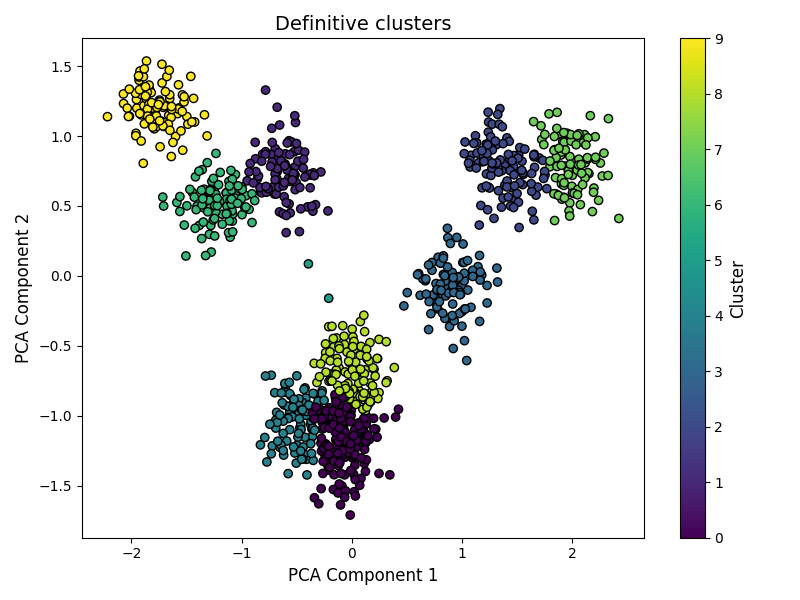
\includegraphics[width=\textwidth]{../data/plots/synthetic_noise_blobs_blobs_A-Link_structural_0.png}
        \caption{A-Link (0.8482)}
    \end{subfigure}
    \begin{subfigure}[b]{0.3\textwidth}
        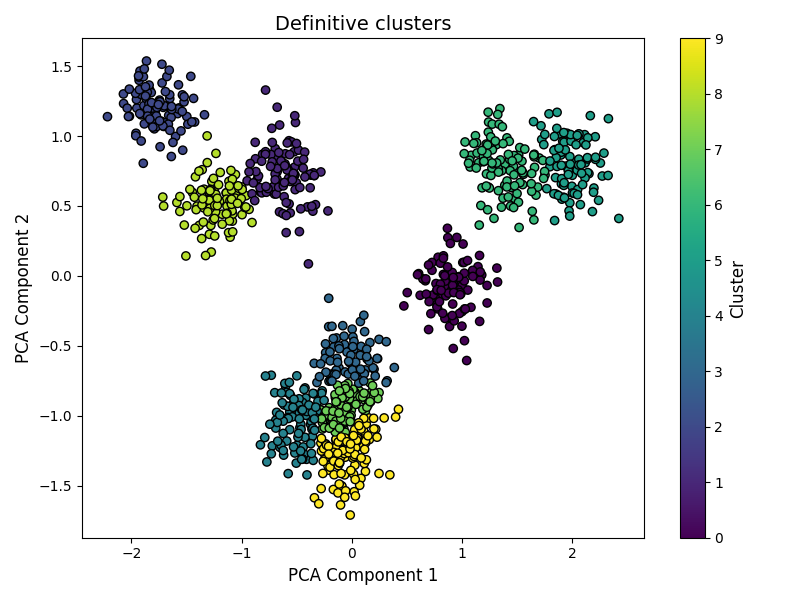
\includegraphics[width=\textwidth]{../data/plots/synthetic_noise_blobs_blobs_PIC_structural_0.png}
        \caption{PIC (0.8429)}
    \end{subfigure}
    \begin{subfigure}[b]{0.3\textwidth}
        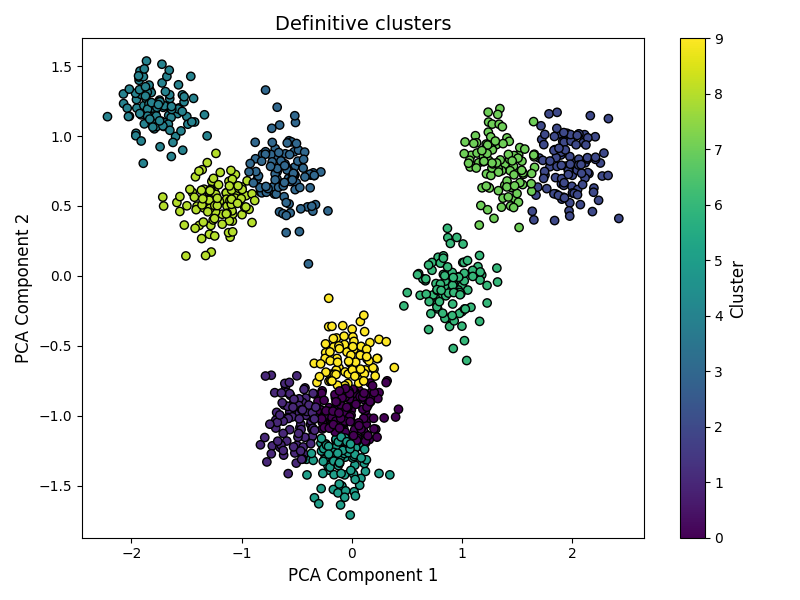
\includegraphics[width=\textwidth]{../data/plots/synthetic_noise_blobs_blobs_Zell_structural_0.png}
        \caption{Zell (0.8403)}
    \end{subfigure}
    
    \vspace{0.3cm}
    
    \begin{subfigure}[b]{0.3\textwidth}
        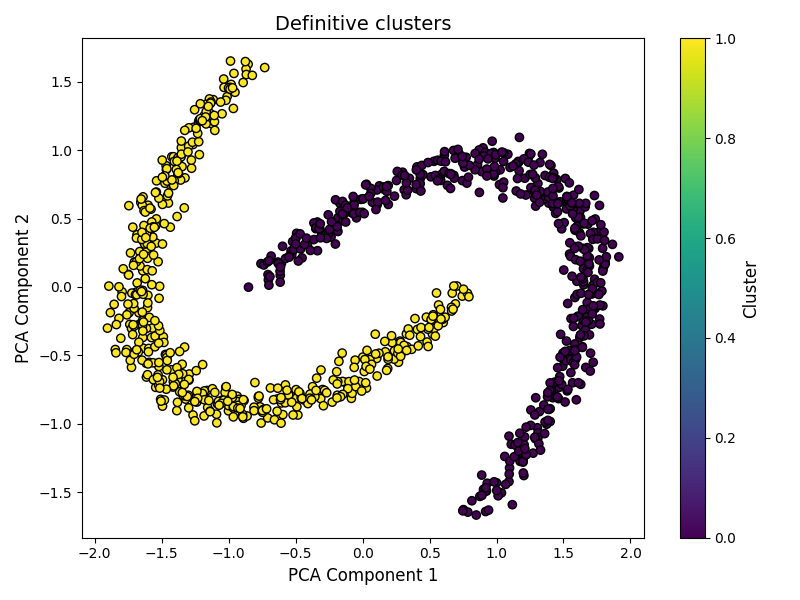
\includegraphics[width=\textwidth]{../data/plots/synthetic_noise_moons_moons_PIC_structural_0.png}
        \caption{PIC (1.0)}
    \end{subfigure}
    \begin{subfigure}[b]{0.3\textwidth}
        \includegraphics[width=\textwidth]{../data/plots/synthetic_noise_moons_moons_A-link_structural_0.png}
        \caption{A-Link (1.0)}
    \end{subfigure}
    \begin{subfigure}[b]{0.3\textwidth}
        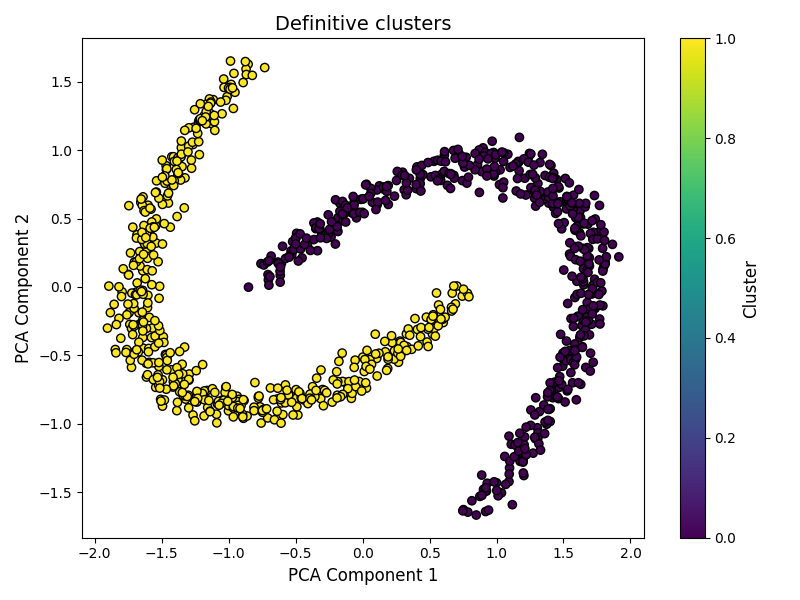
\includegraphics[width=\textwidth]{../data/plots/synthetic_noise_moons_moons_S-link_structural_0.png}
        \caption{S-Link (1.0)}
    \end{subfigure}
    
    \vspace{0.3cm}
    
    \begin{subfigure}[b]{0.3\textwidth}
        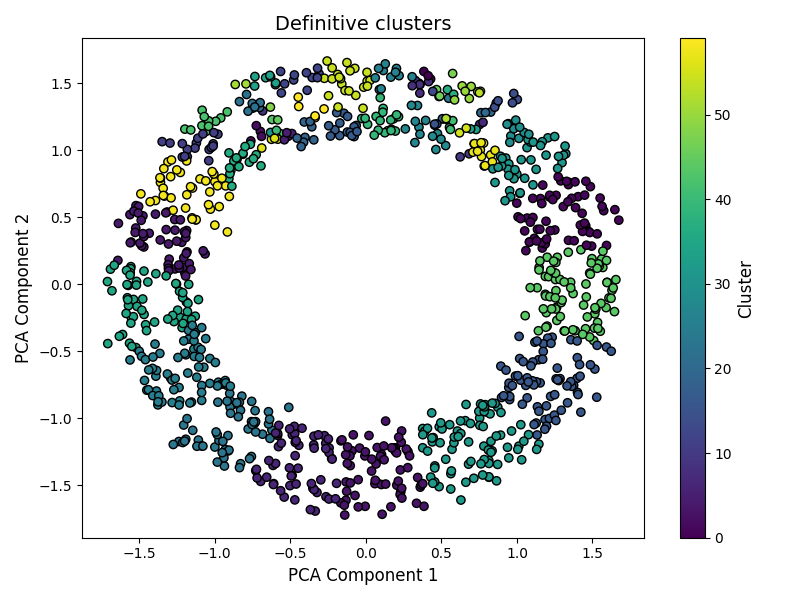
\includegraphics[width=\textwidth]{../data/plots/synthetic_noise_circles_circles_AP_structural_0.png}
        \caption{AP (0.083)}
    \end{subfigure}
    \begin{subfigure}[b]{0.3\textwidth}
        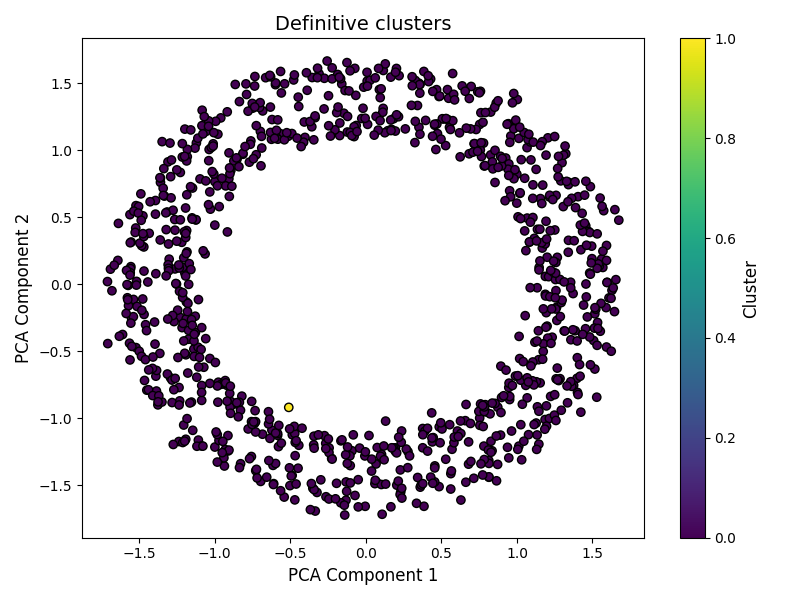
\includegraphics[width=\textwidth]{../data/plots/synthetic_noise_circles_circles_S-link_structural_0.png}
        \caption{S-Link (0.002)}
    \end{subfigure}
    \begin{subfigure}[b]{0.3\textwidth}
        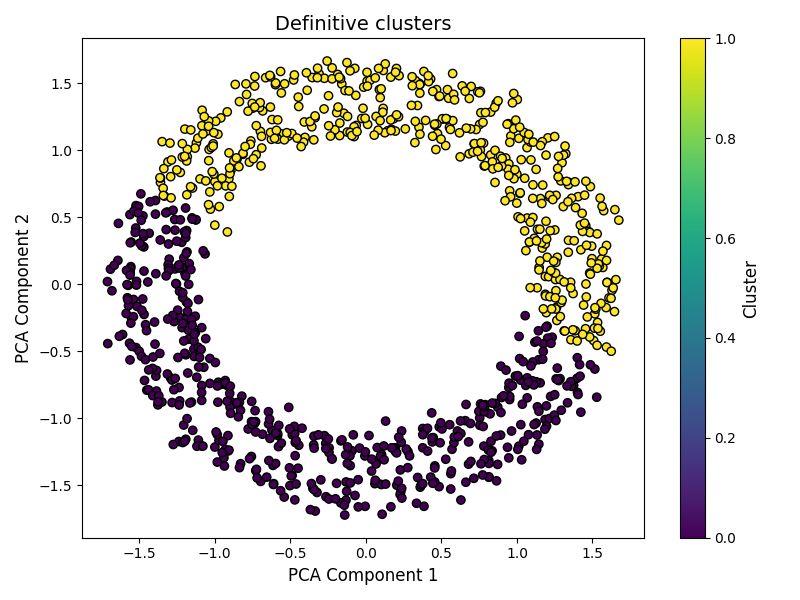
\includegraphics[width=\textwidth]{../data/plots/synthetic_noise_circles_circles_D-kernel_structural_0.png}
        \caption{D-kernel (0.00023)}
    \end{subfigure}

    \caption{Clustering results on the three synthetic datasets. Between parentesis, the NMI score for the algorithm presented on the respective dataset.}
    \label{fig:synthetic_results_grid}
\end{figure}

The results obtained from the synthetic datasets reveal several interesting patterns. In the case of the first dataset, blobs — shown in images (a), (b), and (c) of Figure \ref{fig:synthetic_results_grid} — all algorithms performed well, with the top three achieving nearly identical results, each surpassing 0.84 in Normalized Mutual Information (NMI).

For the second dataset, results indicate that while three algorithms managed to perfectly separate the data, suggesting the dataset is not particularly challenging, the remaining algorithms showed significantly weaker performance. This disparity can be attributed to the specific characteristics and structure of the dataset, which may not align well with the assumptions of those methods.

The third dataset, circles, proved to be the most difficult for the evaluated algorithms. As similarity-based clustering methods, the algorithms struggled to capture the circular structure inherent in the data, resulting in consistently poor performance. In this case, the best-performing algorithm was Affinity Propagation (AP), though its NMI score of 0.08 can not be seen as a good result, as is represented in Figure \ref{fig:synthetic_results_grid}.

Compared to the results reported in the original paper, ours are not as distinctly favorable toward the PIC algorithm. Nevertheless, it remains evident that PIC consistently performs well on both the first and second datasets. However, similar to the other algorithms evaluated, PIC struggles with the third dataset, showing its common limitation when dealing with data of this structure.

\subsection{Algorithm comparison}

This section presents a comparative analysis of our clustering algorithms across the three non-synthetic datasets: USPS, MNIST and BC-Wisconsin, similarly as done in the original paper. The results are summarized in Table \ref{tab:synthetic_results} and Table \ref{tab:synthetic_results}. The first table presents the results in terms of Normalized Mutual Information (NMI), while the second one shows the clustering error.

\begin{table}[h]
    \centering
    \caption{Quantitative clustering results in NMI. The best values are in bold.}
    \begin{tabular}{lcccccccc}
    \toprule
    \textbf{Dataset} & \textbf{USPS} & \textbf{MNIST} & \textbf{BC-W} & \textbf{Blobs} & \textbf{Moons} & \textbf{Circles} \\
    \midrule
    AP       & 0.5176   & 0.4170 & 0.2596 & 0.8028  & 0.2772 & \textbf{0.0831} \\
    A-link   & 0.01128  & 0.0016 & 0.0151 & \textbf{0.8482}  & \textbf{1.0} & 0.0 \\
    S-link   & 0.0019   & 0.0016 & 0.0102 & 0.7067  & \textbf{1.0} & 0.002 \\
    C-link   & 0.1592   & 0.0016 & 0.0102 & 0.8225  & 0.5640 & 0.0 \\
    Zell     & 0.5743   & \textbf{0.6293} & \textbf{0.5679} & 0.8404   & 0.0677 & 0.0001 \\
    D-kernel & 0.2455   & 0.0038 & 0.0102 & 0.8262   & 0.5616 & 0.0002 \\
    PIC & \textbf{0.8708} & 0.0063 & 0.0102 & 0.8430   & \textbf{1.0} & 0.00005 \\
    \bottomrule
    \end{tabular}
    \label{tab:synthetic_results}
\end{table}

\begin{table}[h]
    \centering
    \caption{Quantitative clustering results in Clustering error.The best values are in bold.}
    \begin{tabular}{lccccc}
    \toprule
    \textbf{Dataset} & \textbf{USPS} & \textbf{MNIST} & \textbf{BC-Wisconsin} \\
    \midrule
    AP       & 0.9272   & 0.9527 & 0.8963\\
    A-link   & 0.8285  & 0.7785 & 0.3673  \\
    S-link   & 0.8328   & 0.7785 & 0.3691\\
    C-link   & 0.7634   & 0.7785 & 0.3691\\
    Zell     & 0.4450   & \textbf{0.3592} & \textbf{0.0844}\\
    D-kernel & 0.6698   & 0.7772 & 0.3691\\
    PIC & \textbf{0.1150} & 0.7772 & 0.3691 \\
    \bottomrule
    \end{tabular}
\end{table}

The Normalized Mutual Information (NMI) metric quantifies the similarity between clustering assignments and ground truth labels, where higher values indicate better alignment. According to the original paper, the Path Integral Clustering algorithm outperformed the rest on the USPS and MNIST datasets. However, the current implementation and evaluation reveal some notable differences.

On the USPS dataset, PIC indeed achieves the highest NMI value of 0.8708, very far from the rest of the algorithms, confirming the original paper's claim and proving its strong performance in capturing the underlying cluster structure in a somewhat challenging dataset, considering we are clustering written numbers solely using the pixels. The NMI result presented by the original paper was 0.825 which is very close to the one we obtained, and this is a good indicator that our implementation is working correctly.

For MNIST, on the other hand, we are presented with a significant divergence from the paper's findings. While PIC is reported as the top performer in the original study, it achieves only 0.0063 NMI here, with Zell clearly outperforming it at 0.6293. This inversion suggests that in this replication, either PIC struggled to converge to meaningful clusters, or its assumptions were not well-suited to the MNIST data in this particular implementation. It could also imply that Zell, perhaps under different parameter settings or with the specific MNIST preprocessing used here, was better able to exploit the dataset's structure.

On BC-Wisconsin, which was not reported in the original paper, Zell again clearly leads with an NMI of 0.5679, followed by AP at 0.2596. All other methods, including PIC, performed very poorly here, indicating that Zell may be particularly effective in handling this dataset's cluster characteristics — likely benefitting from its capacity for detecting more globally separated clusters, as seen in the CH scores of table \ref{tab:CH}.

\begin{table}[h]
    \centering
    \caption{Quantitative clustering results in Silhouette score}
    \begin{tabular}{lccccc}
    \toprule
    \textbf{Dataset} & \textbf{USPS} & \textbf{MNIST} & \textbf{BC-Wisconsin} \\
    \midrule
    AP       & 0.077   & 0.0558 & 0.0870 \\
    A-link   & 0.2806  & \textbf{0.7832} & 0.6339  \\
    S-link   & 0.3089   & \textbf{0.7832} & \textbf{0.6606} \\
    C-link   & 0.1945   & \textbf{0.7832} & \textbf{0.6606} \\
    Zell     & 0.0681   & -0.0389 & 0.3263 \\
    D-kernel & \textbf{0.6698}   & 0.6349 & \textbf{0.6606} \\
    PIC      & 0.1390  & 0.5941 & \textbf{0.6606} \\
    \bottomrule
    \label{tab:Silhouette}
    \end{tabular}
\end{table}

\begin{table}[h]
    \centering
    \caption{Quantitative clustering results in DBI}
    \begin{tabular}{lccccc}
    \toprule
    \textbf{Dataset} & \textbf{USPS} & \textbf{MNIST} & \textbf{BC-Wisconsin} \\
    \midrule
    AP       & 1.8701   & 1.5212 & 1.3622 \\
    A-link   & 1.1553  & \textbf{0.1325} & 0.6798 \\
    S-link   & \textbf{0.4623}   & \textbf{0.1325} & \textbf{0.4497} \\
    C-link   & 2.4111   & \textbf{0.1325} & \textbf{0.4497} \\
    Zell     & 2.0193   & 3.3001 & 1.3537 \\
    D-kernel & 2.1858   & 3.0414 & \textbf{0.4497} \\
    PIC     & 2.3121    & 1.5937 & \textbf{0.4497} \\
    \bottomrule
    \end{tabular}
    \label{tab:DBI}
\end{table}

\begin{table}[h]
    \centering
    \caption{Quantitative clustering results in Calinski-Harabasz}
    \begin{tabular}{lccccc}
    \toprule
    \textbf{Dataset} & \textbf{USPS} & \textbf{MNIST} & \textbf{BC-Wisconsin} \\
    \midrule
    AP       & 68.3675   & 25.6472 & 39.0207 \\
    A-link   & 22.2013  & 52.8586 & 32.4822   \\
    S-link   & 4.5830   & 52.8586 & 27.8726 \\
    C-link   & 242.2214   & 52.8586 & 27.8726 \\
    Zell     & \textbf{697.2199}   & \textbf{185.1767} & \textbf{258.9817} \\
    D-kernel & 337.163   & 46.1865 & 27.8726 \\
    PIC      & 517.6182 & 27.6675 & 27.8726 \\
    \bottomrule
    \end{tabular}
    \label{tab:CH}
\end{table}

The Silhouette Score, which measures how similar an object is to its own cluster compared to other clusters, revealed that on the MNIST dataset, the A-link, S-link, and C-link methods all achieved identical and notably high scores of 0.7832. This indicates that these methods produced clusters with a high degree of compactness and separation. On the USPS dataset, the D-kernel method outperformed others with a Silhouette Score of 0.6698, suggesting it formed well-defined clusters in this setting. For the BC-Wisconsin dataset, the S-link, D-kernel, and PIC methods all tied with a strong score of 0.6606.

When considering the Davies-Bouldin Index (DBI), where lower values signify better clustering, consistent patterns are found. On the USPS dataset the S-link method achieves the lowest DBI at 0.4623, outperforming other algorithms in terms of minimizing intra-cluster variance while maximizing inter-cluster separation. For the BC-Wisconsin dataset, the S-link, C-link, D-kernel, and PIC methods shared a DBI value of 0.4497, proving their effectiveness. Zell, D-kernel, and PIC generally performed worse in this metric on MNIST and USPS, despite competitive performances elsewhere.

The Calinski-Harabasz Index (CHI), which rewards high between-cluster dispersion and low within-cluster dispersion, offered a contrasting perspective. The Zell method achieved exceptionally high CHI scores on all three real datasets, particularly on BC-Wisconsin, where it recorded a value of 258.98 clearly surpassing other algorithms. On the USPS dataset, Zell again led with a CHI of 697.22, followed by PIC and D-kernel with notable but lower scores. Although Zell consistently achieved high CHI values, it did not perform as well in the Silhouette and DBI metrics, suggesting that while it can create globally dispersed clusters, they might lack local compactness.

In summary, the results highlight that S-link and A-link methods exhibit balanced, reliable performance across all datasets and metrics, making them strong general-purpose and fast clustering techniques. The D-kernel method excels particularly on the USPS dataset if we only look at internal metrics, while Zell demonstrates outstanding performance in terms of global cluster dispersion (as measured by CHI) but falls behind in terms of compactness and separation as captured by the Silhouette and DBI scores.

That being said, when using internal metrics to evaluate clustering results on labeled data, it's essential to keep in mind that these metrics evaluate the inherent structure of the clustering, without considering the true labels. They do not directly indicate how well the clusters align with the predefined classes, which means an algorithm can achieve strong internal scores while still poorly matching the actual labels — especially if the data's natural structure doesn't correspond to the given categories. The results observed here illustrate this situation clearly.

Nonetheless, internal metrics remain valuable even in labeled scenarios as ours, as they provide complementary information about the structure of the data and quality of the formed clusters. Using internal metrics can help detect situations where the labeled classes themselves might not reflect the underlying structure of the data, or where an algorithm achieves high label agreement through overfitting or by forming poorly separated clusters. In this sense, combining internal and external metrics offers a more complete and reliable assessment than the one presented in the original paper.

We see that for our particularly implemented PIC algorithm, internal metrics show mixed results across the different datasets. In terms of Silhouette score, PIC performs relatively well on BC-Wisconsin, achieving the highest score of 0.6606, but fares worse on USPS and MNIST, with scores of 0.1390 and 0.5941, respectively. The DBI values reflect a similar trend, where PIC has the highest value of 2.3121 on USPS, suggesting less distinct clusters, while it performs better on BC-Wisconsin, with a DBI of 0.4497, indicating more compact and well-separated clusters. As for Calinski-Harabasz, PIC achieves high values on USPS (517.6182) and BC-Wisconsin (27.8726), but struggles on MNIST, with a low value of 27.6675. These results indicate that while the PIC algorithm may generate good clustering quality in some cases, its performance is dataset-dependent, with significant variation in the internal metric scores across different domains.

\subsection{Noise analysis}

In this section we will run experiments using the previously described synthetic dataset incorporating different levels of gaussian noise and structural noise to see how do the different methods behave. Because the addition of gaussian and structural noise is done randomly, we have followed the same practices from the original paper and repeated all the experiments 20 times, showing the mean and the standard deviation at each noise level.

\begin{figure}[h!]
    \centering
    \begin{subfigure}[b]{0.45\textwidth}
        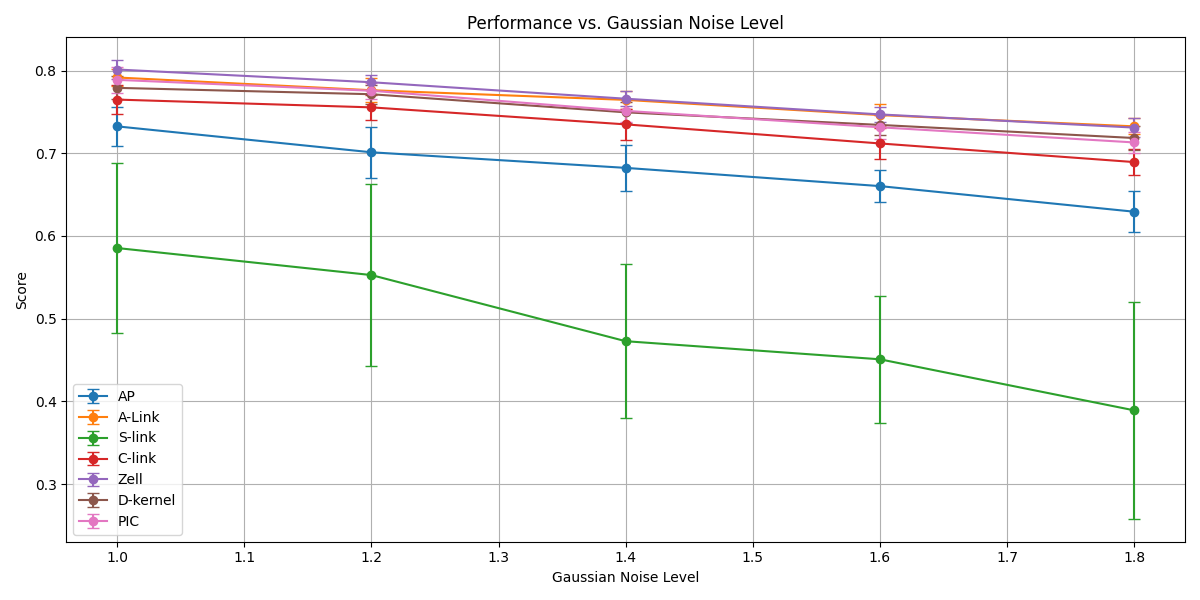
\includegraphics[width=\textwidth]{../data/plots/results_gaussian_noise_blobs.png}
        \caption{Gaussian noise level (Blobs)}
    \end{subfigure}
    \begin{subfigure}[b]{0.45\textwidth}
        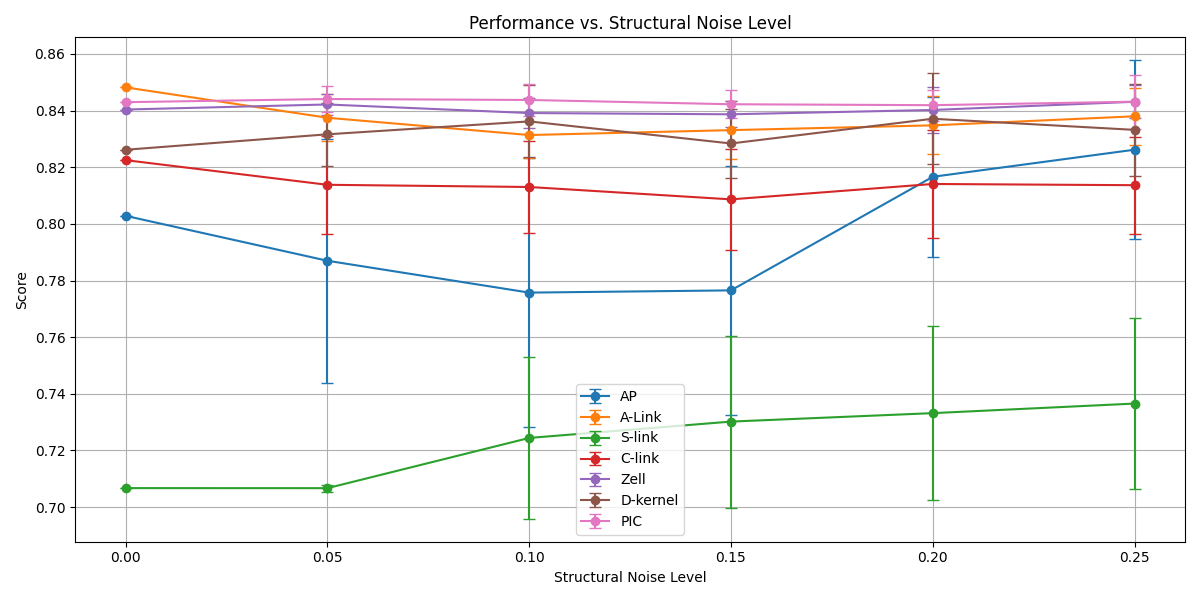
\includegraphics[width=\textwidth]{../data/plots/results_structural_noise_blobs.png}
        \caption{Structural noise level (Blobs)}
    \end{subfigure}
    
    \vspace{0.3cm}
    
    \begin{subfigure}[b]{0.45\textwidth}
        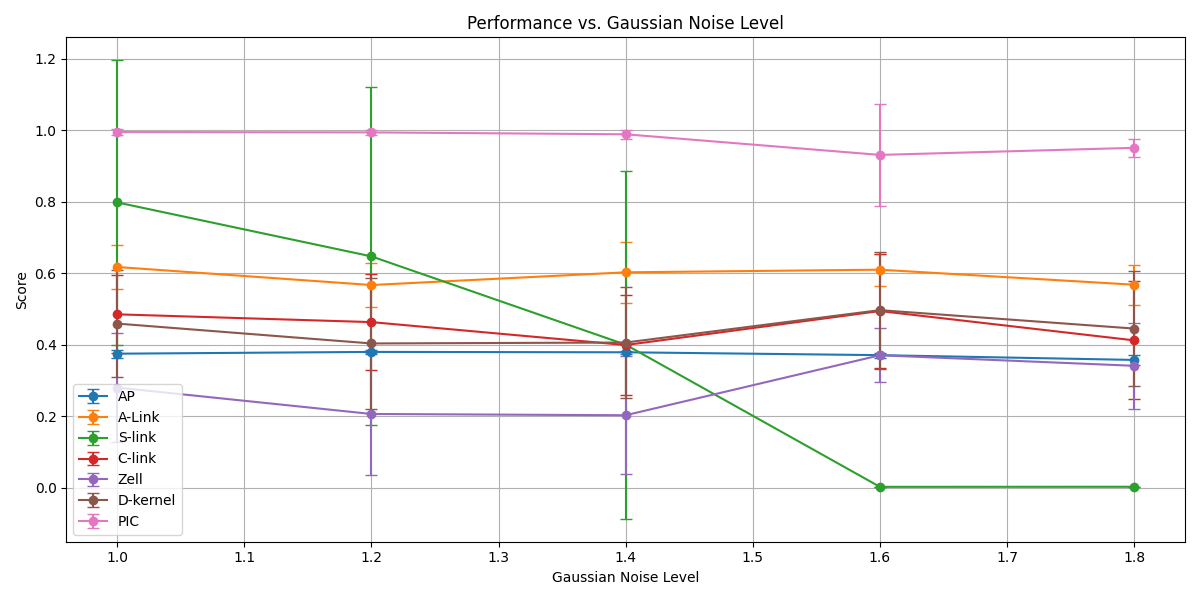
\includegraphics[width=\textwidth]{../data/plots/results_gaussian_noise_moons.png}
        \caption{Gaussian noise level (Moons)}
    \end{subfigure}
    \begin{subfigure}[b]{0.45\textwidth}
        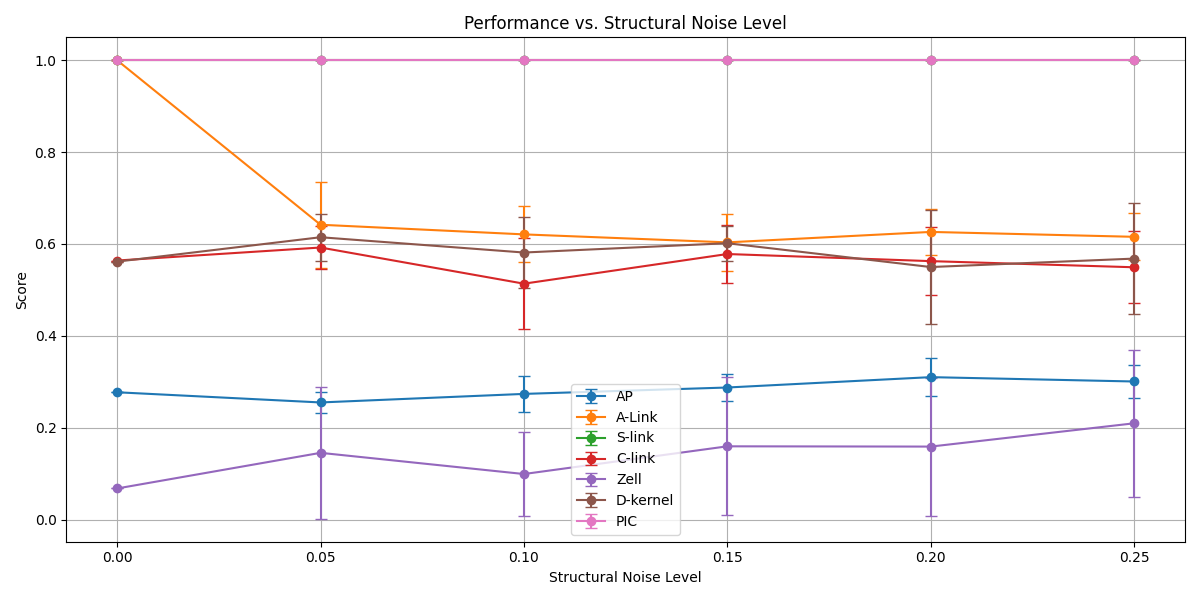
\includegraphics[width=\textwidth]{../data/plots/results_structural_noise_moons.png}
        \caption{Structural noise level (Moons)}
    \end{subfigure}
    
    \vspace{0.3cm}
    
    \begin{subfigure}[b]{0.45\textwidth}
        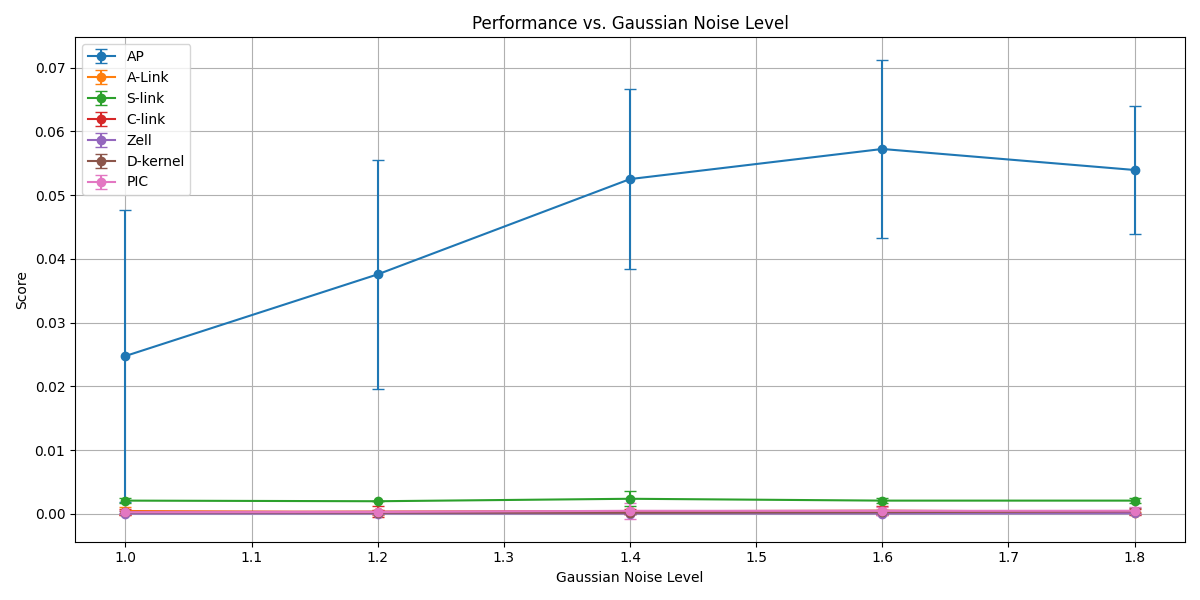
\includegraphics[width=\textwidth]{../data/plots/results_gaussian_noise_circles.png}
        \caption{Gaussian noise level (Circles)}
    \end{subfigure}
    \begin{subfigure}[b]{0.45\textwidth}
        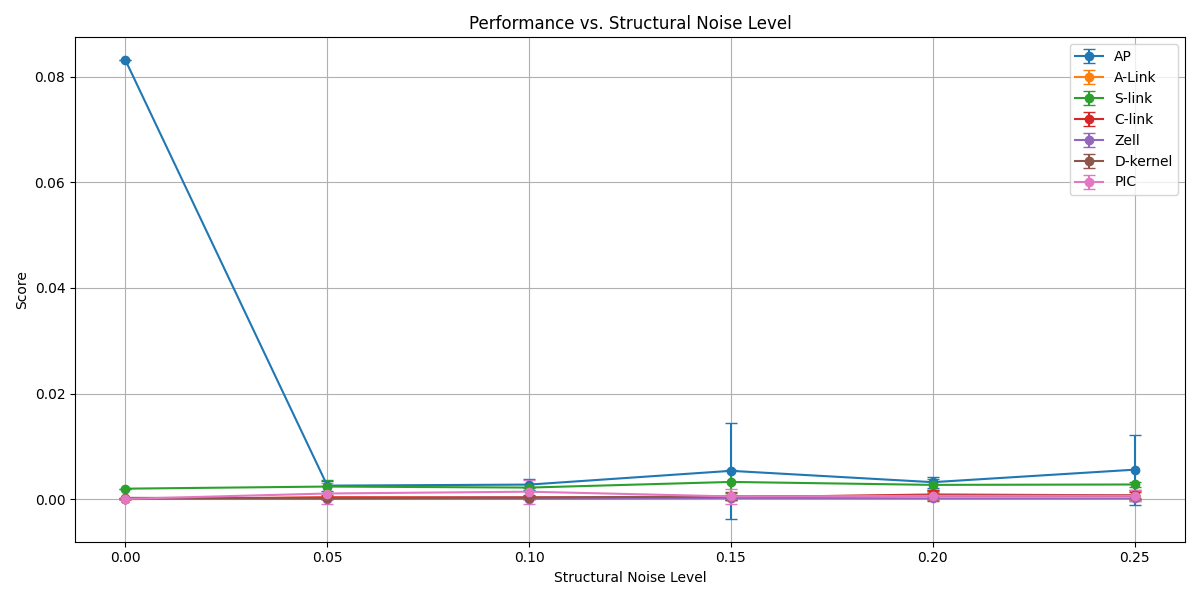
\includegraphics[width=\textwidth]{../data/plots/results_structural_noise_circles.png}
        \caption{Structural noise level (Circles)}
    \end{subfigure}

    \caption{Mean and standard deviation of NMI results for each one of the datasets when applying gaussian noise (left column) and structural noise (right column). Every experiment was repeated 20 times. Structural noise level is defined as the proportion of removed points from the original dataset.}
    \label{fig:noise_analysis}
\end{figure}

For the first dataset, blobs, there is a clear decline on the performance of all algorithms when applying gaussian noise. Despite this overall decline, the relative ranking of the algorithms remains mostly consistent, with each method maintaining its position in comparison to the others throughout the noise levels. Zell is the one that gets the top results at all noise points but the rest of algorithms are very close, with the exception of S-link, AP and C-link, which are clearly performing worse. It is notable to see that the standard deviation of the results is proportional to the NMI scores the algorithms are getting, meaning that the algorithms that are performing better are also more stable.

The structural noise results on the first dataset are very relevant because we can see the resistance of PIC to noise, as stated by the original paper. While most of the algortihms are affected by the structural noise, PIC even increases its NMI score keeping it at over 0.84 with a quarter of the dataset removed. Its standard deviation is also small.

On the second dataset, moons, the results are fully supporting what the paper stated, not only does PIC perform the best, but it also is the most resistant to noise. The gaussian noise almost has no effect on the performance of the algorithm, and the structural noise does not affect it. It is relevant to see how A-link and S-link have a steep decline in score with the addition of noise, showing immense variability between the different runs, while PIC is the only one that manages to keep its score.

On the circles dataset, which we had shown to be more challenging to our algorithms, we see that all of the algorithms perform poorly, with the best one being AP with a score of 0.08. Here we can see a curious effect, with how the addition of gaussian noise has a favorable effect on the AP algorithm, fitting the noise and increasing its NMI score. With the structural noise the opposite happens, and all of the algorithms end up performing equally bad.

In conclusion, we have seen that PIC is the most structural-noise resistant algorithm in our experiments, while having very promising results under the effect of gaussian noise.

\section{Conclusions}

This paper has presented some challenges in the implementation of the Path Integral Clustering algorithm. The unavailability of the original synthetic datasets used in the paper made it difficult to replicate the results. This however permited us to create our own datasts, which were diverse enough to have very varied results that challenged the claims of the paper.

Thanks to the paper's step-by-step development, implementing the Path Integral Agglomerative Clustering was straightforward. Every computation step, constructing the kernel matrix, summing contributions along candidate paths, and normalizing the resulting affinities, was laid out in algorithmic form, so one could follow the derivation without diving into the full formalism of quantum-mechanical path integrals. In practice, this meant we could treat the “path integral” simply as a weighted sum over link sequences, implement the recurrence relations directly, and easily against datasets in minutes. The only aspect left largely to my own judgment was the overall workflow—how to organize data preprocessing, similarity initialization, and merge order—so I experimented with a couple of pipeline layouts before choosing the one reported here.

So, to sum up, although being a challenging algorithm, with the concepts of Path Integral and complex mathematics, we did not find a lot of problems. The main problem  found was regarding the heap, as we tried to dinamically update the clusters that were removed we were modifying the affinities of the wrong clusters, which was hard to detect, and ended up using the approach explained, where a set is used to store the active clusters and a heap to store the affinities. This made the algorithm run in linear time, which was one of the main goals of the project.

Regarding the claims of the paper, we have seen that the PIC algorithm indeed outperforms state-of-the-art clustering algorithms in some datasets, but not in all of them. We have seen that the algorithm is very resistant to structural noise, and that it performs well on the USPS dataset, but it does not perform as well on MNIST, where Zell outperforms it and in addition it takes considerably longer than the algorithms it is being compared to. We have also seen that the algorithm is very resistant to gaussian noise, and that it performs well on some of the datasets. Despite this, in the circles dataset, all of the algorithms perform poorly, and that includes the PIC algorithm.

In conclusion, we have seen that the PIC algorithm is a very promising algorithm, and that it is very resistant to noise, but it does not outperform all of the algorithms in all of the datasets. We have also seen that the implementation of the algorithm is not as hard as it seems, and that it can be done in a short amount of time. We have succeeded in implementing the algorithm and running it on diverse datasets, both included in the paper and not included in the paper, and we have successfully performed an analysis on its performance under diverse conditions of noise and structure.


\newpage
\section{Bibliography}

\renewcommand{\section}[2]{}%
\begin{thebibliography}{9}

\bibitem{citation1}
Wei Zhang et al.,
\textit{Agglomerative clustering via maximum incremental path integral}, 2013
\href{https://www.sciencedirect.com/science/article/pii/S0031320313001830}{(Link)}

\bibitem{citation2}
Javier Béjar,
URL - 2025 Spring Term
\textit{Clustering evaluation and validation}

\end{thebibliography}

\end{document}